% !Mode:: "TeX:UTF-8"
% !TEX program = xelatex
\begin{question}{5.1}{}
    Derive the wave equation for a string that moves in a medium in which the resistance force between the string and the medium is proportional to the velocity of the string.
\end{question}
% Recall that in the derivation of wave equation, we include the external force $F(x,t)$, which is given by $F(x,t)=-ku_t(x,t)$ for some positive constant $k$ in our case here. Therefore, in formula
% \[
%     u_{tt} = a^2u_{xx} + f(x,t) \quad x\in(0,l), t\in(-\infty,\infty),
% \]
% if we replace the term $f(x,t)$ by $-ku_t(x,t)/\rho(x)$, then we obtain the desired equation
% \[
%     u_{tt} = a^2u_{xx} -bu_t \quad x\in(0,l), t\in(-\infty,\infty),
% \]
% where $b=k/\rho$.
\begin{figure}[H]
    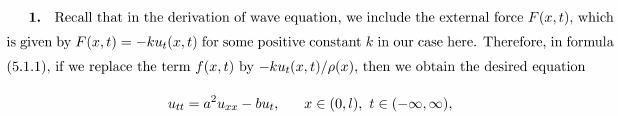
\includegraphics[width=.9\textwidth]{figures/5.1-1.png}
\end{figure}


\begin{question}{5.2}{}
    Solve the following initial-boundary value problems for the wave equation
    \begin{enumerate}[label=(\roman*)]
        \item \[
                \begin{cases}
                    u_{tt} - 4u_{xx} = 0, & x\in(0,1), t\in\RR, \\
                    u(0,t) = u(1,t) = 0, & t\in\RR, \\
                    u(x,0)=\sin(\pi x), u_t(x,0)=\sin(4\pi x), & x\in(0,1). \\
                \end{cases}
            \]
        \item \[
                \begin{cases}
                    u_{tt} - a^2u_{xx} = 0, & x\in(0,1), t\in\RR, \\
                    u_x(0,t) = u_x(1,t) = 0, & t\in\RR, \\
                    u(x,0)=x, u_t(x,0)=0, & x\in(0,1). \\
                \end{cases}
            \]
        \item \[
                \begin{cases}
                    u_{tt} - a^2u_{xx} = 0, & x\in(0,1), t\in\RR, \\
                    u(0,t) = u_x(1,t) = 0, & t\in\RR, \\
                    u(x,0)=0, u_t(x,0)=\cos(\pi x), & x\in(0,1). \\
                \end{cases}
            \]
    \end{enumerate}
\end{question}
\begin{figure}[H]
    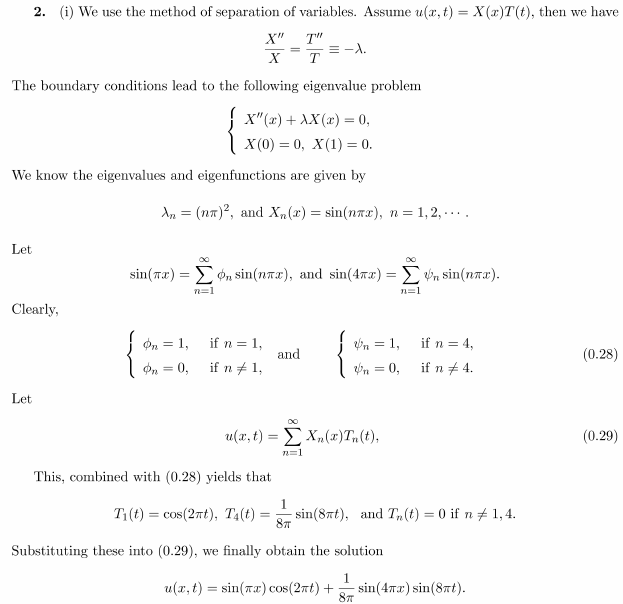
\includegraphics[width=.9\textwidth]{figures/5.2-1.png}
\end{figure}
\begin{figure}[H]
    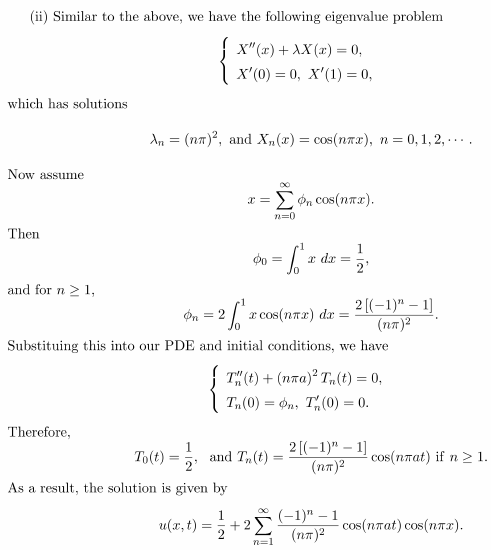
\includegraphics[width=.8\textwidth]{figures/5.2-2.png}
\end{figure}
\begin{figure}[H]
    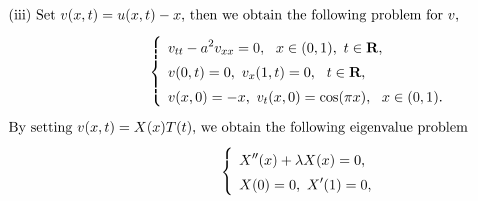
\includegraphics[width=.75\textwidth]{figures/5.2-3.png}
\end{figure}
\begin{figure}[H]
    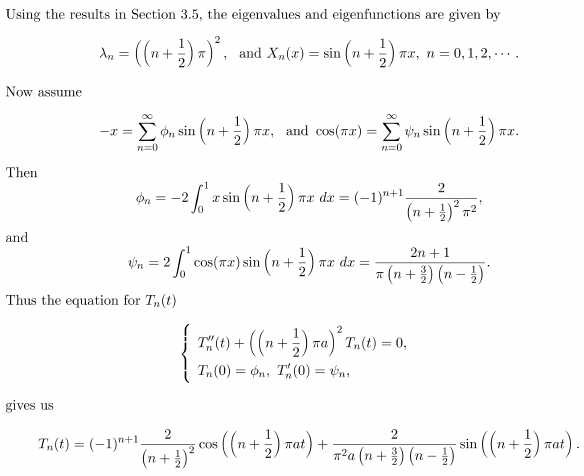
\includegraphics[width=.9\textwidth]{figures/5.2-4.png}
\end{figure}
\begin{figure}[H]
    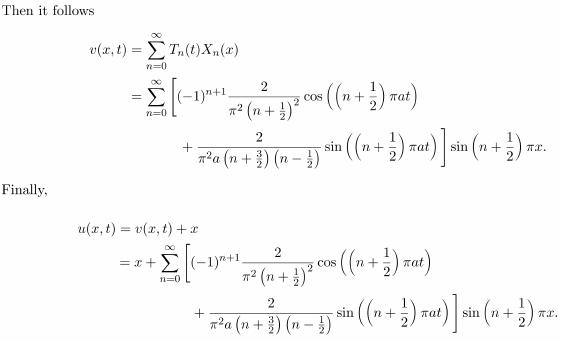
\includegraphics[width=.8\textwidth]{figures/5.2-5.png}
\end{figure}


\begin{question}{5.3}{}
    Solve the Cauchy problem
    \[
        \begin{cases}
            u_{tt} - a^2u_{xx} = 0, & x\in\RR, t\in\RR, \\
            u(x,0)=e^{-x^2}, u_t(x,0)=\sin(x), & x\in\RR. \\
        \end{cases}
    \]
\end{question}
\begin{figure}[H]
    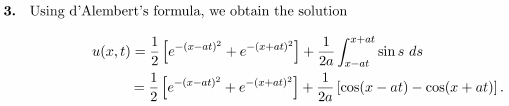
\includegraphics[width=.9\textwidth]{figures/5.3-1.png}
\end{figure}


\begin{question}{5.4}{}
    Solve the Cauchy problem
    \[
        \begin{cases}
            u_{tt} - a^2u_{xx} = 0, & x\in\RR, t\in\RR, \\
            u(x,0)=0, u_t(x,0)=\psi(x), & x\in\RR, \\
        \end{cases}
    \]
    where
    \[
        \psi = \begin{cases}
            1, & \text{for $\abs{x}<a$}, \\
            0, & \text{for $\abs{x}\geq a$}. \\
        \end{cases}
    \]
    Sketch the graph of $u$ vs $x$ at times $t=1/2$,$1$,$3/2$,$2$.
\end{question}
\begin{figure}[H]
    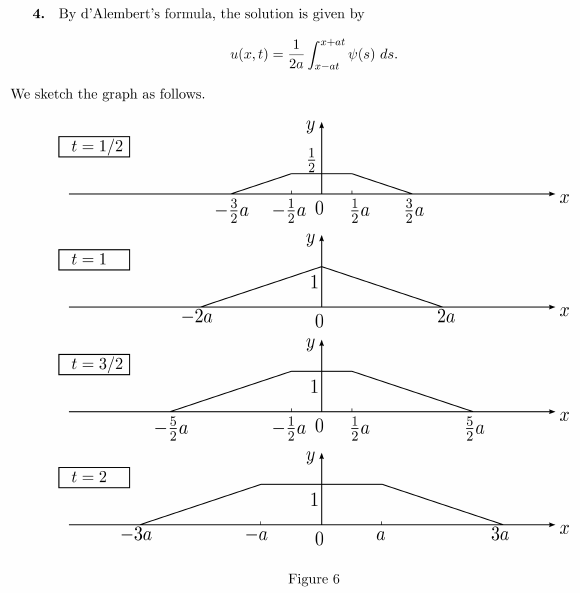
\includegraphics[width=.9\textwidth]{figures/5.4-1.png}
\end{figure}


\begin{question}{5.6}{}
    Let $u$ be the solution of
    \[
        \begin{cases}
            u_{tt} - a^2u_{xx} = 0, & x\in\RR, t\in\RR, \\
            u(x,0)=\phi(x), u_t(x,0)=\psi(x), & x\in\RR. \\
        \end{cases}
    \]
    Show that if both $\phi$ and $\psi$ are even functions, then so is $u$ in $x$. Formulate and prove the analog when both $\phi$ and $\psi$ are odd.
\end{question}
\begin{figure}[H]
    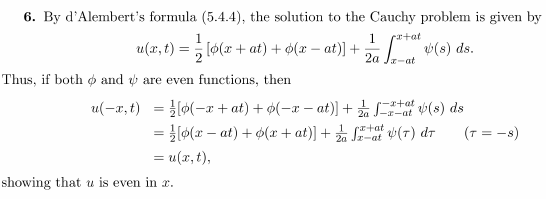
\includegraphics[width=.9\textwidth]{figures/5.6-1.png}
\end{figure}


\begin{question}{5.7 (Bonus) \index{Unsolved}}{}
    Let $u$ be a smooth solution of the wave equation
    \[
        u_{tt} = u_{xx},\quad x\in\RR, t\geq 0.
    \]
    Prove that for any $(x_0,t_0)\in(-\infty,+\infty)\times(0,+\infty)$,
    \[
        \int_{x_0-t_0+t}^{x_0+t_0-t}\frac{1}{2}(u_t^2+u_x^2)(x,t)\dd x \leq \int_{x_0-t_0}^{x_0+t_0}\frac{1}{2}(u_t^2+u_x^2)(x,0)\dd x,
    \]
    for all $t\in(0, t_0)$.\footnote{Hint: multiple the wave equation by $u_t$ and then trying to re-write the equation in the form\[F_t-G_x=0.\] Integrate this equation and apply Green's Theorem to the trapezoid bounded by the x-axis, the characteristic lines passing through $(x_0,t_0$, and the horizontal line at $t$.)}
\end{question}
